\documentclass[compress]{beamer}

\usepackage[utf8]{inputenc}
\usepackage[english]{babel}
\usepackage[alf,abnt-and-type=&]{abntex2cite}
\usepackage{graphicx,hyperref,url,multicol,ragged2e,amsmath,tikz}
\usepackage{framed, color}
\definecolor{shadecolor}{rgb}{1,0.8,0.3}
\DeclareGraphicsExtensions{.pdf,.png,.jpg}
\usepackage[font=footnotesize]{subcaption}
\usepackage[export]{adjustbox}




\mode<presentation>
{
  \setbeamertemplate{background canvas}[vertical shading][bottom=white!10,top=red!10]
%  \usetheme{Berkeley}
 \usetheme{CambridgeUS}
%  \usetheme{Madrid}
%  \usetheme{Warsaw}
  \usefonttheme[onlysmall]{structurebold}
  
  \setbeamertemplate{headline}{}
  
%  \setbeamercovered{invisible} % default
   \setbeamercovered{ transparent, again covered={\opaqueness{25}} } % =15%
%   \setbeamercovered{transparent=50}
%   \setbeamercovered{dynamic}

%   \setbeamercovered{again covered={\opaqueness<1->{25}}}
}

% The title of the presentation:
%  - first a short version which is visible at the bottom of each slide;
%  - second the full title shown on the title slide;
\title[Social Capital Inequalities]{Social Capital Inequalities among Postgraduate Students and Social Selection Processes}

% Optional: a subtitle to be dispalyed on the title slide
%\subtitle{Show where you're from}

% The author(s) of the presentation:
%  - again first a short version to be displayed at the bottom;
%  - next the full list of authors, which may include contact information;
\author[Neylson Crepalde]{
  Neylson Crepalde, PhD Candidate.  \\\medskip
  {\footnotesize \url{neylson.crepalde@izabelahendrix.edu.br}\\ 
  {\footnotesize \url{http://neylsoncrepalde.github.io}}}}

% The institute:
%  - to start the name of the university as displayed on the top of each slide
%    this can be adjusted such that you can also create a Dutch version
%  - next the institute information as displayed on the title slide
\institute[GIARS]{
  Grupo Interdisciplinar de Pesquisa em Análise de Redes Sociais \\ 
  Sociology Department -- UFMG}

% Add a date and possibly the name of the event to the slides
%  - again first a short version to be shown at the bottom of each slide
%  - second the full date and event name for the title slide
\date[2016, June]{
  FAFICH -- 2016, June 30}

\begin{document}

\begin{frame}[plain]
  \titlepage
  
  
  \begin{tikzpicture}[remember picture,overlay] % Background box
  \node [xshift=\paperwidth/2,yshift=\paperheight/6] at (current page.south west)[rectangle,fill,inner sep=0pt,minimum width=\paperwidth,minimum height=\paperheight/8,top color=darkred,bottom color=darkred]{}; % Change the height of the box, its colors and position on the page here
  \end{tikzpicture}
  

   \begin{figure}
    \flushbottom
    
\includegraphics[scale=0.3, valign=t]{GIARS_logo2.png}
   \end{figure}




  
\end{frame}

\begin{frame}
  \frametitle{Conteúdo}

  \tableofcontents
\end{frame}



% Section titles are shown in at the top of the slides with the current section 
% highlighted. Note that the number of sections determines the size of the top 
% bar, and hence the university name and logo. If you do not add any sections 
% they will not be visible.
\section{Introduction}

\begin{frame}
  \frametitle{Introduction}

\justify

  The idea of a fully egalitarian world is an impossible abstraction. As \citeonline{lin1999building} shows, people are born in an already stratified social space where individuals in different positions have different access, and therefore, different mobilizing capacities of their social capital. This is due to individual positioning in social structures, family socioeconomic background, and other person related attributes. This is no news to sociologists. However, the process of social groups formation is not so acknowledged yet although it is central to understand how the access to social resources is achieved. This has only recently been investigated.
 
\end{frame} 

\begin{frame}
\justify

  Here, I intend to show that the concept of social capital has been widely mobilized in a confusing and careless way, specially within studies that deal with educational inequalities. This, according to \citeonline{portes2000two}, can lead to spurious conclusions. I will present a methodological framework that operationalizes the concept very well obtaining many gains in objectivity and reliability, social network analysis.
  
  \vspace{3mm}
  
  Therefore, this paper aims to discuss the inequalities that are held within the academic system, specifically within a social sciences postgraduate program in a Brazilian university. To do this, we will focus our investigation in two main aspects: academic productivity and social ties formation. We used data collected online from 47 social sciences psotgraduate students (masters and doctoral). To perform the analysis, we used linear models, social network analysis, stochastic blockmodelling and the highly modern \textit{social selection model} (SSM).
    
\end{frame}

\section{Social Capital and Inequalities}
\begin{frame}
	\frametitle{Social Capital and Inequalities}
	\justify
	
	\citeonline[p. 35]{lin1999building} defines social capital as ``resources embedded in a social structure which are accessed and/or mobilized in purposive actions''.
	
	\vspace{3mm}
	
	\citeonline{portes1998social} presents an excellent review on the origin and applicability of social capital in sociology. So does \citeonline{higgins2005fundamentos}.
	
	\vspace{3mm}
	
	\begin{quote}
		\footnotesize
		Closure of parental networks is measured by the number of parents of child's friends known to her or his parents; parental school involvement is a composite index of parent's participation in school activities and frequency of meetings with school staff about their child's academic progress. The content of these items correspond closely to Coleman's conceptual description of social capital. \cite[p. 7]{portes2000two}
	\end{quote}
	
\end{frame}


\begin{frame}

	
	\begin{alertblock}{Up to this point,}
	it is easy to perceive that the concept is operationalized in a variety of ways in the literature. In fact, \citeonline[p. 2]{portes2000two} states that ``much of the controversy surrounding social capital has to do with its application to different types of problems and its use in theories involving different units of analysis''.
	\end{alertblock}
	
\end{frame}

\begin{frame}
	\justify
	In his most famous article ``The Strength of Weak Ties'', \citeonline{granovetter1973strength} showed the importance of ``distant'' contacts to have access to new information. According to him, ``from  the  individual's  point  of  view,  then,  weak  ties  are  an  importante resource in making possible mobility opportunity'' \cite[p. 1373]{granovetter1973strength}.
	
	\vspace{3mm}
	
	\citeonline{erickson2001good} develops her paper in close dialogue with Granovetter. She investigates the effect of social capital on the hiring process focusing both on employee and employer. The main point of the article is that regardless of the contact point by which the job was taken, having a good social capital will lead to better jobs and better pay.
\end{frame}


\subsection{Social Capital and Education}
\begin{frame}
	\frametitle{Social Capital and Education}
	
	\justify
	
	\citeonline[p. 110]{silva2003expansao} studies educational stratification within the brazilian educational expansion context. It is curious, though, that the mobilization of the variable \textit{female householder} as a proxy of social capital does not seem a good choice because it is based on a highly questionable assumption (that families with a female householder have poorer social capital) and it does not tell us anything apparently relevant about tie mobilization and its resources.
	
	\vspace{3mm}
	
	\citeonline{mont2011estratificaccao} applied multinomial logistic regression models to understand the completion of secondary school and entering university. Unfortunately, the author used the same variable (\textit{female householder}) as a proxy of social capital without any discussion on the subject. Indeed, the only place he mentions social capital is on the articles abstract.
\end{frame}


\begin{frame}
	\justify
	
	\citeonline{silva2000tendencias} also use \textit{female householder} along with the number of \textit{14 or less years old children} in the families studied, the percentage of \textit{mothers that work} and whether \textit{children from 10 to 14 years old work} or not.
	
	\vspace{3mm}
	
	\begin{alertblock}{Although}
		the authors are worried about explaining the social context of the chosen variables, why are they good indexes for social capital or not is never discussed.
	\end{alertblock}
	
	In short, \textit{the main argument} I want to delineate in this section is that this concept has been widely and inadvertently used. I believe that the most useful tool to handle it is social network analysis by which social capital can be objectly measured using a repertoire of indexes like Burt's constraint, centrality measures (both indexes for popularity and activity within a given group), structural equivalence and modelled using up-to-date statistical techniques.
\end{frame}


\section{Data and Methods}
\begin{frame}
	\frametitle{Data and Methods}
	
	\justify
	
	In conducting this research, data from 47 postgraduate students was collected through an online survey in May, 2016. This sample represents 60\% of the total number of students enrolled in a postgraduation program at a Brazilian university. For the purpose of the analysis conducted here, we will assume this group as a ``complete network''.
	
	\vspace{3mm}
	
	The developed questionnaire had four parts.The first was an invitation and an agreement term with which the subjects must have agreed to proceed to the questions. In the second part, the subjects were questioned about personal and socialeconomic information. In the third part, they were questioned about their academic life, productivity and impressions. In the last part, the sociometric part, they were present to the complete list of grad colleagues and they were asked to indicate persons regarding 6 issues: scientific collaboration, paper reviewing, theoretical and methodological advisement, friendship and professional indication.
\end{frame}

\begin{frame}
	\begin{figure}[!ht]
		\centering
		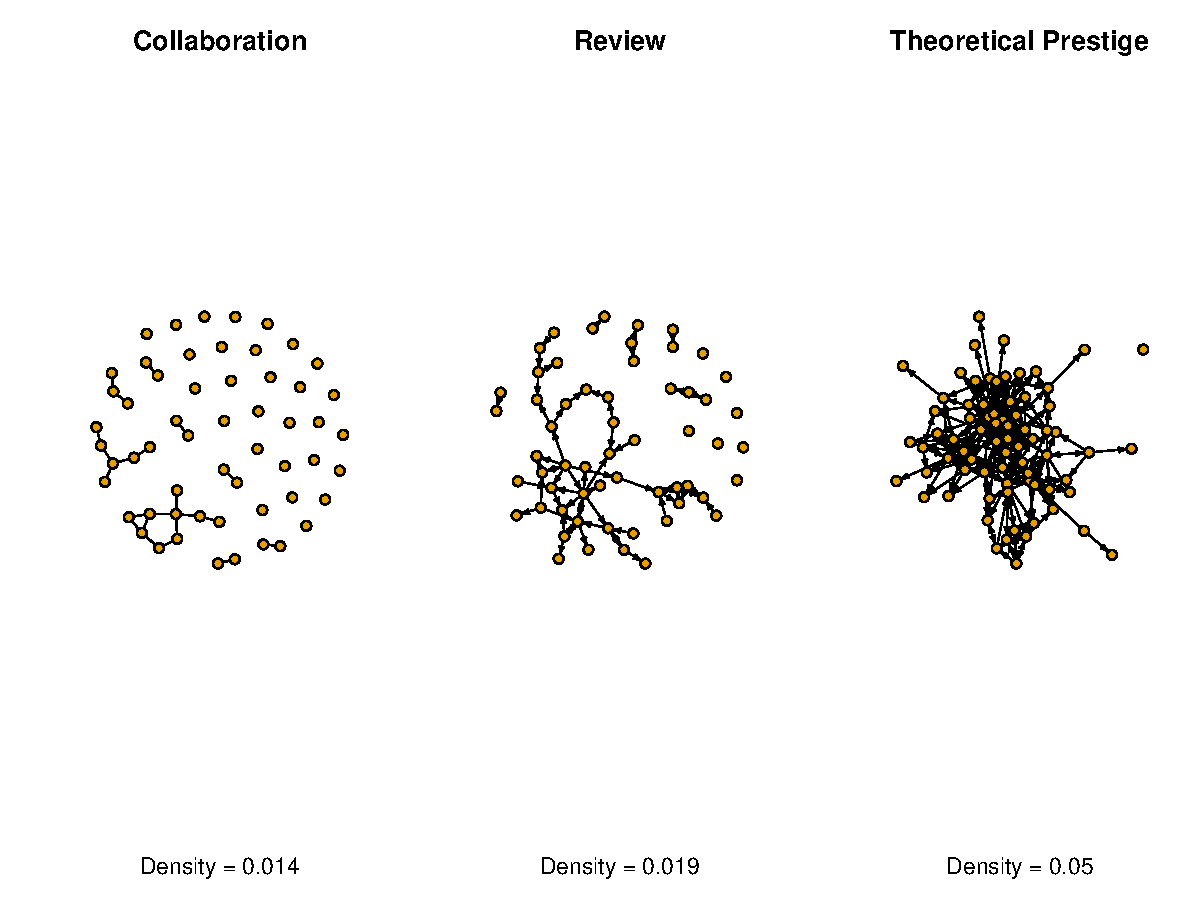
\includegraphics[scale=0.5]{redes1.pdf}
	\end{figure}
\end{frame}

\begin{frame}
	\begin{figure}[!ht]
		\centering
		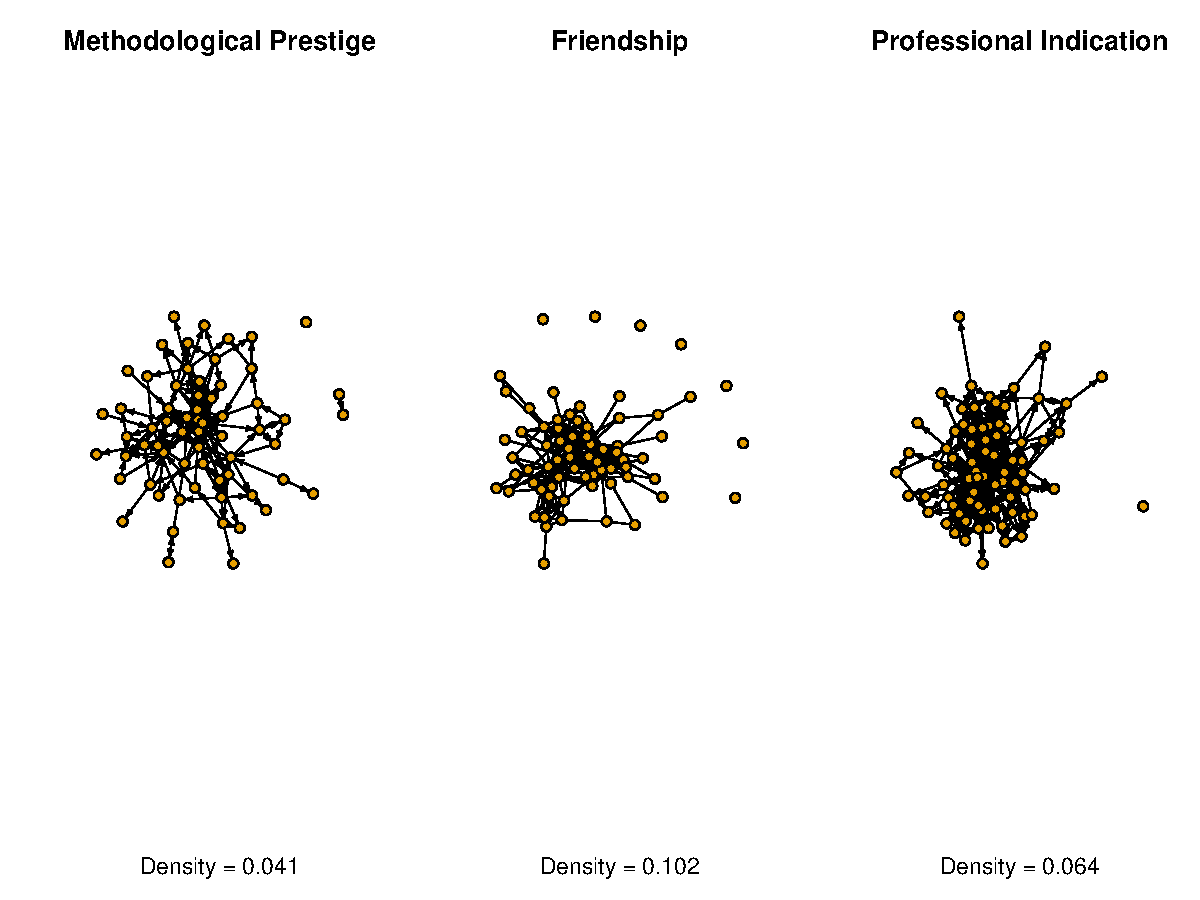
\includegraphics[scale=0.5]{redes2.pdf}
	\end{figure}
\end{frame}


\begin{frame}
	\justify
	
	To perform the analysis, social network analysis metrics were used as well as a statistic model from the \textit{exponential random graph models} family, or p* models.
	
	\vspace{3mm}
	
	The p* model can be defined by
	
	\begin{equation}
	Pr(Y=y) \quad = \quad \left(\frac{1}{k}\right) exp \left\{ \sum_{A} \eta_A g_A (\textbf{y}) \right\}
	\end{equation}
	
	where Y is the theoretical estimated graph, y is the observed graph, $\sum_{A}$ is the summation of all configurations \textit{A},  $\eta_A$ is the estimated parameter corresponding to the configuration \textit{A}, $g_A(\textbf{y})$ is the network statistic corresponding to the configuration \textit{A} of the graph \textbf{y} and \textit{k} is a constant which ensures the proper probability distribution.
\end{frame}


\begin{frame}
\justify

Here, I use an extension of the p* models known as \textit{Social Selection Model} (SSM). The SSM was proposed by \citeonline{robins2001network} with the goal of accounting for heterogeneity within the social structures using nodal attributes as exogenous covariates.

I also analyze the effect of dyadic covariates, i.e., the effect of the existence of an \textit{i--j} tie in another relation network on the existence of an \textit{i--j} tie in the modelled network.
\end{frame}

\section{Results}
\begin{frame}
	\frametitle{Results -- Individual related variables}
	
	\begin{table}[ht]
			\centering
			\caption{Descriptive Statistics - Quantitative}
			\label{quanti}
		
		\begin{tabular}{p{4cm}p{4cm}}
				\hline
				Age & Income (R\$) \\ 
				\hline
				Min.   : 23   & Min.   :   0   \\ 
				1st Qu.: 27   & 1st Qu.: 1500   \\ 
				Median : 29   & Median : 2200   \\ 
				Mean   : 30.32 & Mean   : 2636   \\ 
				3rd Qu.: 33   & 3rd Qu.: 3000   \\ 
				Max.   : 43   & Max.   : 8200   \\ 
				\hline
			\end{tabular}
		
	\end{table}
\end{frame}

\begin{frame}
	\begin{table}[ht]
			\centering
			\scriptsize
			\caption{Descriptive Statistics - Qualitative (\%)}
			\label{quali}
		
		\begin{tabular}{rrrrr}
				\hline
				Gender & Race & Formal Work & Academic situation & Scholarship \\ 
				\hline
				Female: 63,83   & White: 55.32   & No: 63.83  & Doctor: 06.38   & No: 29.79 \\ 
				Male: 36,17      & Mestizo: 02.13   & Yes: 36.17 & Doctorate Std.: 51.06  & Yes: 70.21 \\ 
				& Dark Skinned: 02.13   &  & Master Std.: 40.43 &  \\ 
				& Black: 04.26   &  & Master: 02.13 &  \\ 
				& Brown: 36.17   &  &  &  \\ 
				\hline
			\end{tabular}
		
	\end{table}
\end{frame}

\begin{frame}
	\begin{table}[ht]
			\centering
			\footnotesize
			\caption{Occupations}
			\label{occupations}
		
		\begin{tabular}{lrr}
				\hline
				& Frequency & Percentage \\ 
				\hline
				Research Assistant &   1 & 2.13 \\ 
				Social Worker &   1 & 2.13 \\ 
				Housewife &   1 & 2.13 \\ 
				Student &  29 & 61.70 \\ 
				Researcher &   3 & 6.38 \\ 
				Professor &   5 & 10.64 \\ 
				Psychologist &   1 & 2.13 \\ 
				Government Employee &   2 & 4.26 \\ 
				Sociologist &   4 & 8.51 \\ 
				Total &  47 & 100.00 \\ 
				\hline
			\end{tabular}

	\end{table}
\end{frame}

\begin{frame}
	\begin{figure}[hbt]
		\centering
		\caption{Self-evaluation}
		\label{self-evaluation}
		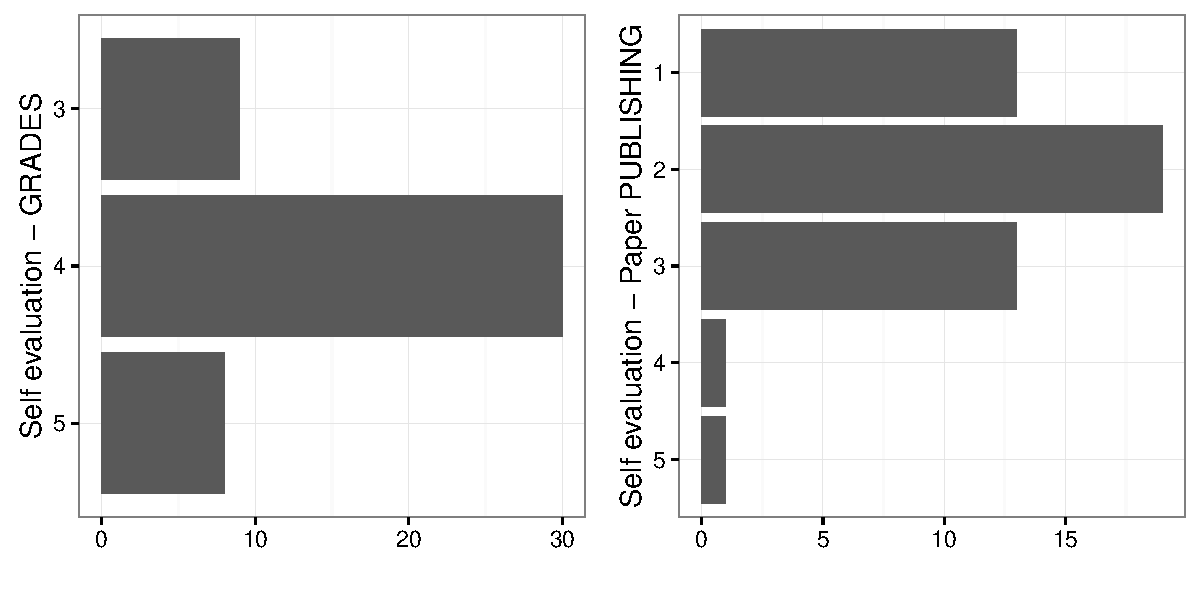
\includegraphics[scale=0.5]{autoavaliacoes.pdf}
	\end{figure}
\end{frame}

\begin{frame}
	\begin{figure}[ht]
		\centering
		\caption{Productivity}
		\label{productivity}
		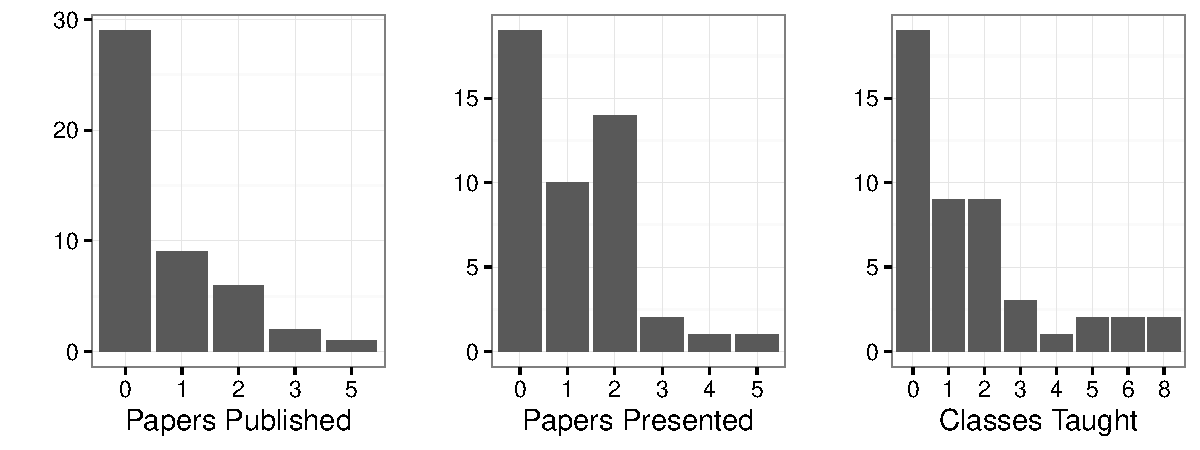
\includegraphics[scale=0.5]{pub_con_classes.pdf}

	\end{figure}
\end{frame}

\begin{frame}
	\begin{table}[ht]
			\centering
			\scriptsize
			\caption{Correlations}
			\label{correlations}
		
		\begin{tabular}{r|cccccccc}
				\hline
				& Age & Income & Grades & Pubs & Papers & Congress & Classes & Prod. \\ 
				\hline
				Age & 1.00 &  &  &  &  &  &  &  \\ 
				Income & 0.39 & 1.00 &  &  &  &  &  &  \\ 
				Grades & -0.19 & -0.03 & 1.00 &  &  &  &  &  \\ 
				Pubs & 0.09 & 0.16 & 0.32 & 1.00 &  &  &  &  \\ 
				Papers & -0.01 & 0.12 & 0.09 & 0.54 & 1.00 &  &  &  \\ 
				Congress & 0.16 & 0.19 & 0.24 & 0.49 & 0.57 & 1.00 &  &  \\ 
				Classes & 0.21 & 0.45 & -0.16 & 0.15 & 0.18 & 0.07 & 1.00 &  \\ 
				Prod. & 0.16 & 0.37 & 0.04 & 0.53 & 0.82 & 0.65 & 0.66 & 1.00 \\ 
				\hline
			\end{tabular}
		
	\end{table}
\end{frame}

\begin{frame}
\justify
To investigate if age, income, scholarship and occupation have an effect on academic productivity within the studied universe, I estimated two linear models, one by OLS and a Generalized Linear Model with gamma distribution and identity link, with the following specification:

\begin{multline}
\label{linear}
\widehat{Productivity} = \beta_0 + \beta_1ResearchGroup + \beta_2Gender + \beta_3White + \\ \beta_4Self Eval(Pub) + \beta_5Age(centralized) + \beta_6Work + \beta_7Income + \\ \beta_8Scholarship + \epsilon
\end{multline}

\end{frame}

\begin{frame}
	\begin{table}
		\centering
		\scriptsize
			\caption{Regression Models}
			\label{linear-coefficients}
		
		\begin{tabular}{l c c }
				\hline
				& Model 1 & Model 2 \\
				& (OLS)   & (GLM -- Gamma) \\
				\hline
				Intercept    & $-1.14 \; (2.17)$     & $0.19 \; (1.88)$      \\
				Research Group (Yes) & $0.86 \; (1.06)$      & $1.52 \; (0.91)$      \\
				Gender (Male)  & $0.43 \; (1.17)$      & $-0.38 \; (0.71)$     \\
				White (Yes)    & $0.70 \; (1.06)$      & $0.79 \; (0.73)$      \\
				Self-eval (Pub)    & $1.93 \; (0.60)^{**}$ & $1.80 \; (0.54)^{**}$ \\
				Age (centralized)     & $0.00 \; (0.12)$      & $0.13 \; (0.10)$      \\
				Work (Yes)  & $-1.69 \; (1.37)$     & $-1.43 \; (0.89)$     \\
				Income     & $0.00 \; (0.00)^{*}$  & $0.00 \; (0.00)$      \\
				Scholarship (Yes) & $-0.52 \; (1.34)$     & $-0.55 \; (0.99)$     \\
				\hline
				R$^2$          & 0.41                  &                       \\
				Adj. R$^2$     & 0.29                  &                       \\
				Num. obs.      & 47                    & 47                    \\
				RMSE           & 3.33                  &                       \\
				AIC            &                       & 238.57                \\
				BIC            &                       & 257.07                \\
				Log Likelihood & -118.29               & -109.29               \\
				Deviance       & 422.34                & 19.16                 \\
				\hline
				\multicolumn{3}{l}{\scriptsize{$^{***}p<0.001$, $^{**}p<0.01$, $^*p<0.05$}}
			\end{tabular}
		\end{table}
\end{frame}

\begin{frame}
	\begin{table}[ht]
			\centering
			\footnotesize
			\caption{Likelihood Ratio Test}
			\label{lrtest}
		
		\begin{tabular}{lrrrrr}
				\hline
				& \#Df & LogLik & Df & Chisq & Pr($>$Chisq) \\ 
				\hline
				OLS & 10 & -118.29 &  &  &  \\ 
				GLM (Gamma) & 10 & -109.29 & 0 & 18.01 & 0.0000 \\   
				\hline
			\end{tabular}
	\end{table}
\end{frame}

\subsection{Relational Data}
\begin{frame}
	\frametitle{Relational Data}
	
	\begin{figure}[htb]
		\centering
		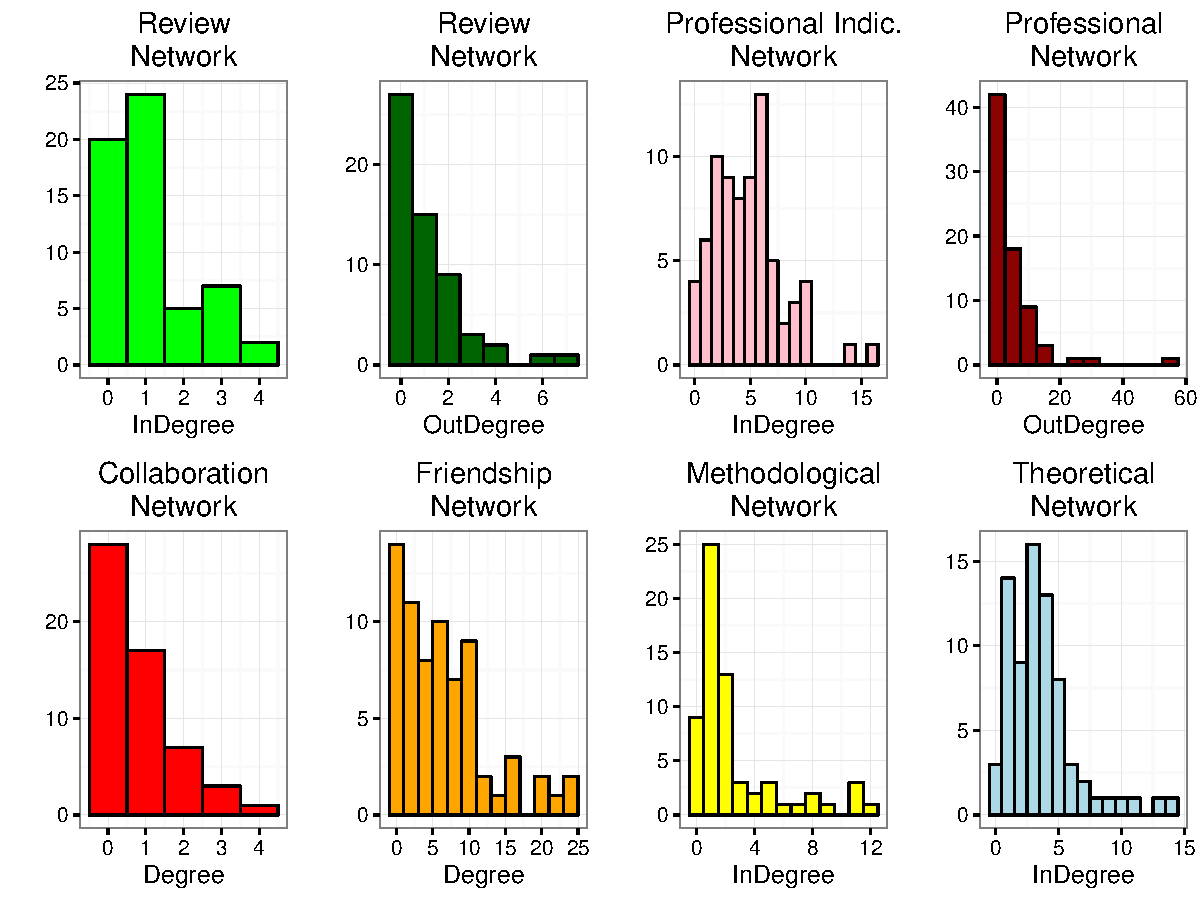
\includegraphics[scale=0.5]{degree_distributions.pdf}
	\end{figure}
\end{frame}

\begin{frame}
	\justify
	
	I estimated again the generalized linear model presented in equation \ref{linear} with ``log'' link and the gamma distribution and including centrality measures for the collaboration, review (in) and methodological (in) networks, one at a time; although no one of them had a significant effect, again, the p-value here is not relevant. The exponential coefficients for these measures were $Cent(Collaboration) = 1.17$, $Cent(Review) = 1.10$ and $Cent(Methodological) = 1.00$ showing that people who collaborate tend to be more productive. The same is applied to people who are regarded as methodologically competent.
	
\end{frame}

\subsection{Collaboration and association among postgraduate students}
\subsubsection{Stochastic Blockmodel}
\begin{frame}
	\frametitle{Stochastic Blockmodel}
	\begin{figure}[ht]
		\centering
		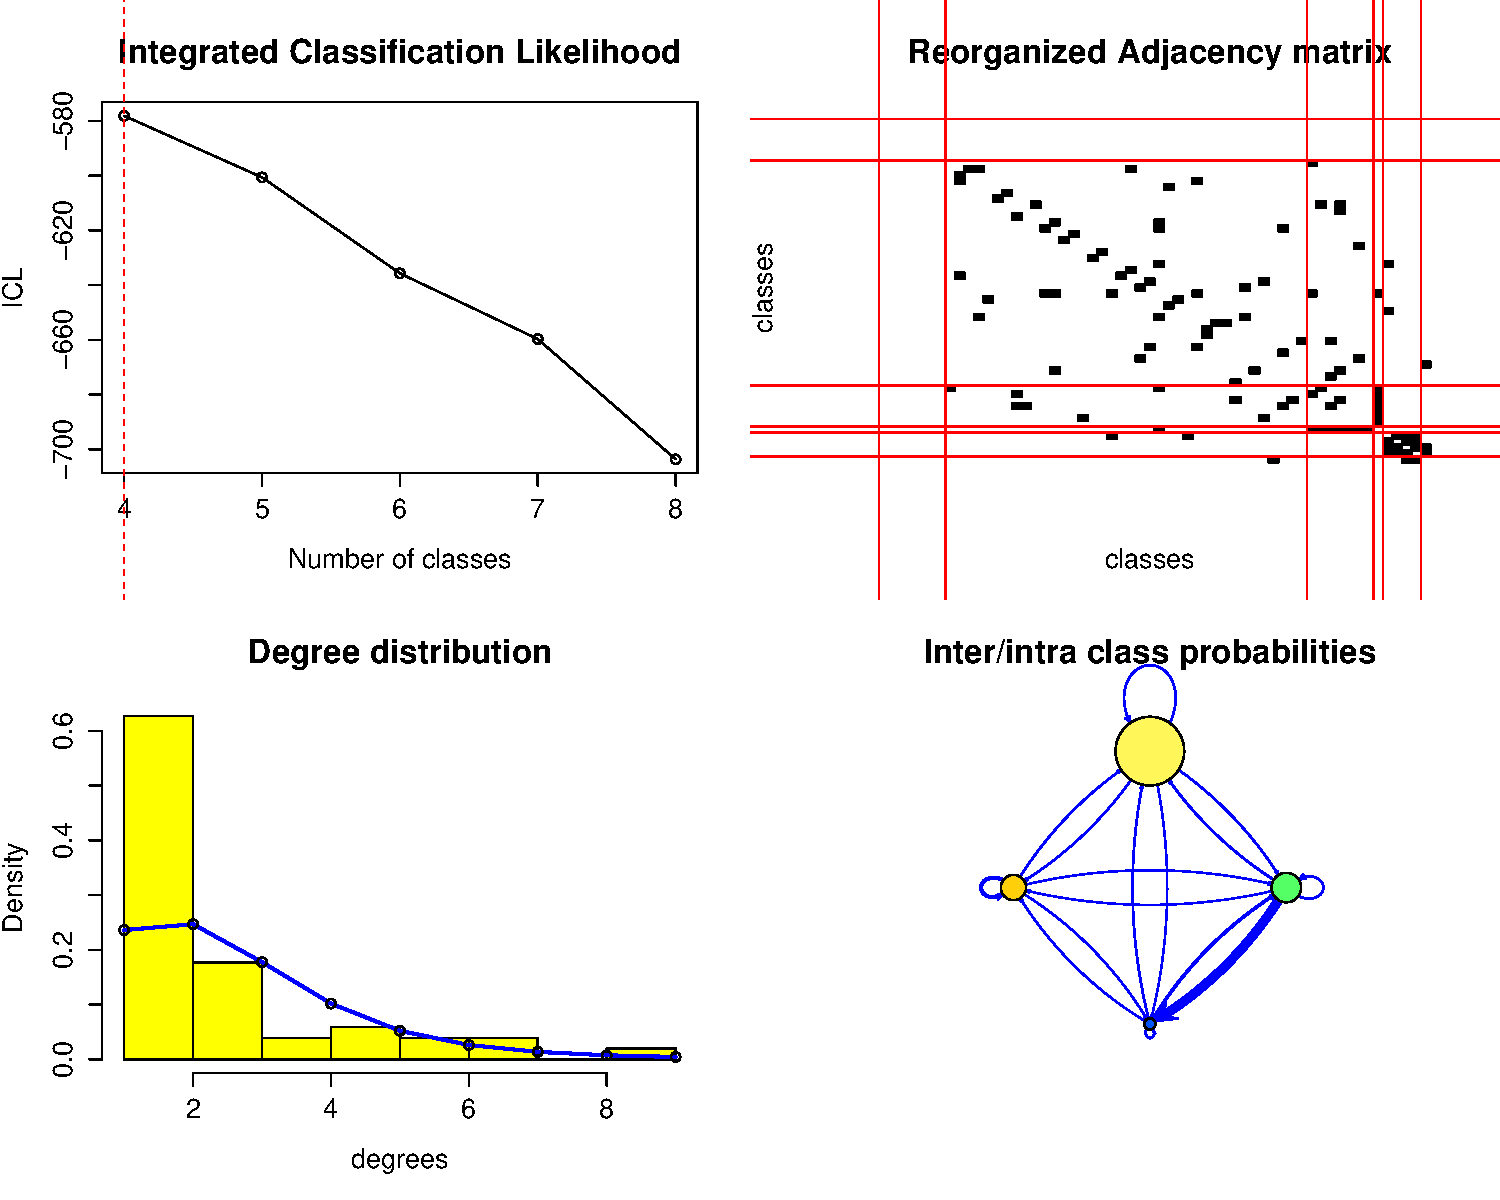
\includegraphics[scale=.4]{block_out.pdf}
	\end{figure}
\end{frame}

\begin{frame}
	\begin{figure}[h]
		\centering
		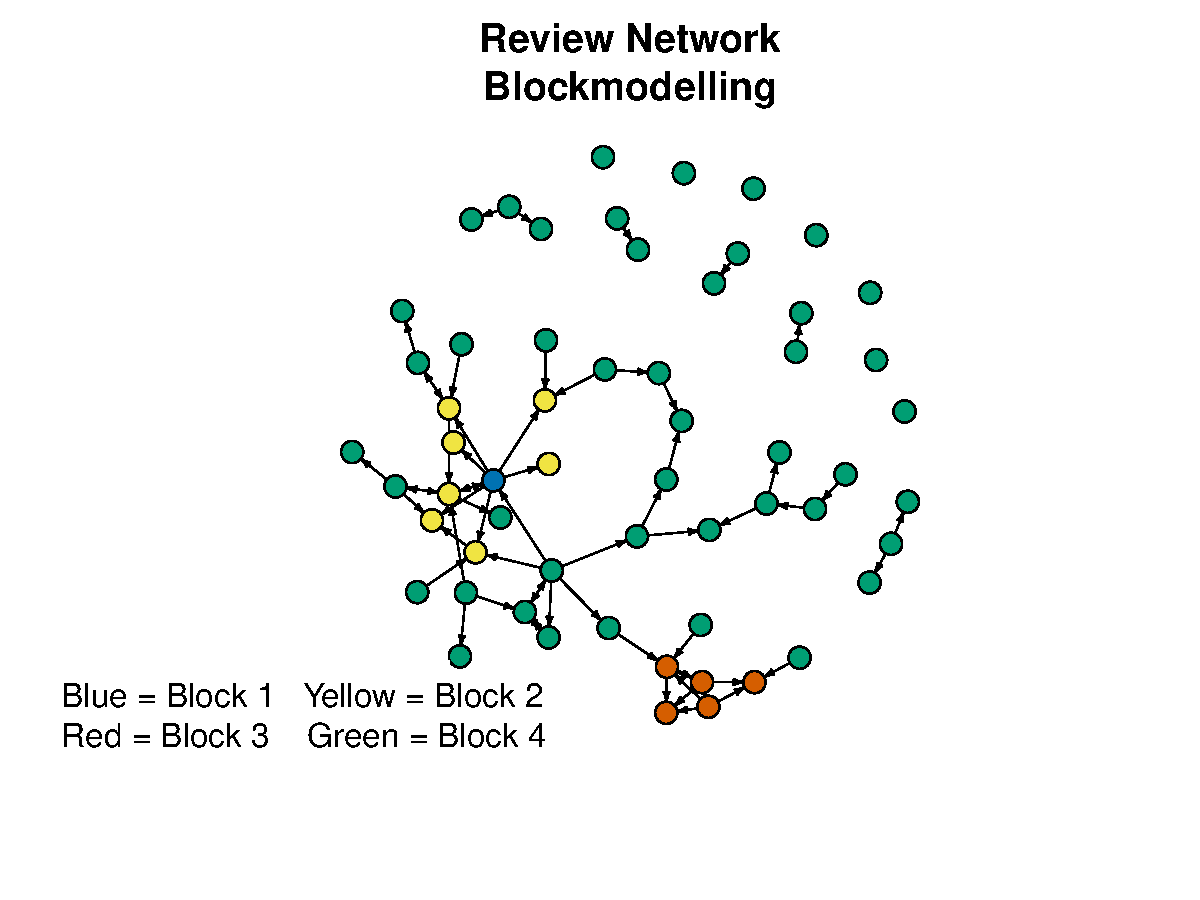
\includegraphics[scale=.6]{net_block.pdf}
	\end{figure}
\end{frame}

\subsubsection{Social Selection Model}
\begin{frame}
	\frametitle{Social Selection Model}
	
	\begin{table}[!h]
			\centering
			\tiny
			\caption{ERGM's -- Dependent: \textbf{Collaboration Network}}
			\label{ergm_colab}
		
		\begin{tabular}{l c c c }
				\hline
				& Model 1 & Model 2 & Model 3 \\
				&         & (ERGM) & (SSM) \\
				\hline
				\textbf{Purely structural effects} & & & \\
				Edges  				  & $-4.56 \; (0.28)^{*}$ & $-4.05 \; (1.10)^{*}$ & $-4.22 \; (0.13)^{*}$ \\
				Isolates              &                         & $0.52 \; (0.74)$        & $0.37 \; (0.22)$        \\
				Triangulation (gwesp) &                         & $1.04 \; (0.36)^{*}$   & $1.07 \; (0.29)^{*}$  \\
				Conectivity(twopath)  &                         & $-0.16 \; (0.29)$       & $-0.14 \; (0.15)$       \\
				\textbf{Covariate network effects} & & & \\
				Review net            & $1.81 \; (0.70)^{*}$   & $1.87 \; (0.68)^{*}$   & $2.31 \; (0.14)^{*}$  \\
				Theoretical net       & $0.40 \; (0.66)$        & $0.40 \; (0.65)$        & $0.54 \; (0.14)^{*}$  \\
				Methodological net    & $1.26 \; (0.68)$        & $1.27 \; (0.66)$        & $1.24 \; (0.13)^{*}$  \\
				Professional Indic. net & $0.81 \; (0.52)$        & $0.73 \; (0.50)$        & $0.65 \; (0.23)^{*}$   \\
				Friendship net        & $-0.46 \; (0.67)$       & $-0.50 \; (0.66)$       & $-0.54 \; (0.09)^{*}$ \\
				\textbf{Actor-relation effects} & & & \\
				Same Research Group        &                         &                    & $1.94 \; (0.29)^{*}$  \\
				Homophily (Gender)        &                         &                     & $-0.65 \; (0.12)^{*}$ \\
				Homophily (White)         &                         &                     & $-0.73 \; (0.31)^{*}$   \\
				Absolute Difference (Productivity) &            &                         & $-0.00 \; (0.05)$       \\
				Absolute Difference (Income)       &            &                         & $0.00 \; (0.00)$        \\
				\hline
				AIC                   & 223.33                  & 220.81                  & 220.26                  \\
				BIC                   & 255.15                  & 268.54                  & 294.51                  \\
				Log Likelihood        & -105.66                 & -101.41                 & -96.13                  \\
				\hline
				\multicolumn{4}{l}{\scriptsize{$^*significant$ (Wald test)}}
			\end{tabular}
	\end{table}
\end{frame}


\section{Discussion}
\begin{frame}
	\frametitle{Discussion}
	
	\justify
	
	James \citeonline{moody2004structure} stated that the scientific collaboration network in social sciences is moved by research specialty and that ``quantitative work is more likely to be coauthored than non-quantitative work''. In this research we found the same pattern with the difference that it was not the research specialty itself that connects students but, essencialy, the research groups.
	
	\vspace{3mm}
	
	 The SSM showed that methodological habilities lead to collaboration more than theoretical ones. This is in consonance with Moody's findings about quantitative work. In fact, the research groups that appear in the blockmodel are essentially quantitative researchers.
	 
	 \vspace{3mm}
	 
	 The linear models did not present big productivity differences by gender, race or income. In this sense, a postgraduate program seems to provide equal opportunities for all its students, once they are in. The models pointed for the centrality of research groups to productivity.
\end{frame}

\begin{frame}
	\justify
	
	A quite amazing finding is that scholarship students are less productive than non-scholarship ones. This deserves deeper investigation for it contrasts all university funding policies.

	\vspace{3mm}
	
	Finally, I hope to have shown the strength of social network analysis on the operationalization of social capital. Although I have addressed a different area from the educational inequalities articles reviewed, I could deal with the same concept, i.e., ``resources embedded in a social structure which are accessed and/or mobilized in purposive actions'' \cite[p. 35]{lin1999building} in a more straightfoward and objective way. We can actually visualize the social structure and mathematically measure popularity, social positioning and social roles. The educational inequalities field would gain a lot with the use of this methodological framework and a more reflexive way of thinking on social capital.
\end{frame}


% contracapa

\begin{frame}

\begin{tikzpicture}[remember picture,overlay] % Background box
\node [xshift=\paperwidth/2,yshift=\paperheight/2] at (current page.south west)[rectangle,fill,inner sep=0pt,minimum width=\paperwidth,minimum height=\paperheight/3,top color=darkred,bottom color=darkred]{}; % Change the height of the box, its colors and position on the page here
\end{tikzpicture}
% Text within the box
\begin{center}
\vspace{14mm}
\color{white}\sffamily
{\bfseries\LARGE Thank you.\par} % Thank you
\vspace{6mm}
\end{center}
\begin{center}
	\begin{figure}
    
\includegraphics[scale=0.3, valign=t]{GIARS_logo2.png}
    \end{figure}
   \vfill
\end{center}


\end{frame}


\bibliography{BIBSEA}
\end{document}